\section{Clasificadores}
Como clasificadores, he decidido entrenar modelos de regresión logística y
perceptrón multicapa. Cabe destacar que he intentando entrenar otros modelos
como \textit{Random Forest} o SVM, pero era incapaz de ello ya que RStudio se
encontraba siempre con algún error fatal que hacía abortar la sesión.

En las siguientes secciones, se va a explicar cómo se ha llevado a cabo el
entrenamiento de los modelos usando el paquete \textit{caret} y, también, se
compararán los resultados de cada uno para cada conjunto de datos de los dos que
hemos preparado.

Antes de entrenar cualquier modelo, los datos se dividen en dos subconjuntos
para entrenamiento y validación usando la función
\lstinline{createDataPartition()} de \textit{caret}. En mi caso, un 70\% se
destina a entrenamiento y, el resto, a validación.

\begin{lstlisting}
library(caret)

set.seed(0)

# ROSE
train_index_rose <- createDataPartition(data_balanced_rose$isFraud, p = .7, list = FALSE)
train_rose <- data_balanced_rose[train_index_rose, ]
val_rose <- data_balanced_rose[-train_index_rose, ]

# SMOTE
train_index_smote <- createDataPartition(data_balanced_smote$isFraud, p = .7, list = FALSE)
train_smote <- data_balanced_smote[train_index_smote, ]
val_smote <- data_balanced_smote[-train_index_smote, ]
\end{lstlisting}

\subsection{Regresión logística}
A pesar de su nombre, la regresión logística es una técnica muy utilizada en
problemas de clasificación binaria, como es el caso del nuestro. Esta técnica se
apoya en la función sigmoide, la cuál nos proporciona un valor entre 0 y 1, que
interpretamos como la probabilidad de que se pertenezca a la clase principal.

He decidido usar este clasificador debido a que es muy simple y no requiere de
un gran consumo de recursos, lo cuál favorece su entrenamiento en mi ordenador
personal, donde se ha realizado la práctica.

\begin{lstlisting}
# ROSE
lr_grid_rose <- expand.grid(.nIter = 5)
lr_control_rose <- trainControl(method = "repeatedcv", number = 10, repeats = 5)
lr_model_rose <- train(
  isFraud ~ .,
  data = train_rose,
  method = "LogitBoost",
  trControl = lr_control_rose,
  tuneGrid = lr_grid_rose
  )

lr_prediction_rose <- predict(lr_model_rose, val_rose, type = "raw")

# SMOTE
lr_grid_smote <- expand.grid(.nIter = 5)
lr_control_smote <- trainControl(method = "repeatedcv", number = 10, repeats = 5)
lr_model_smote <- train(
  isFraud ~ .,
  data = train_smote,
  method = "LogitBoost",
  trControl = lr_control_smote,
  tuneGrid = lr_grid_smote
)

lr_prediction_smote <- predict(lr_model_smote, val_smote, type = "raw")
\end{lstlisting}

Como se puede ver en el código, los clasificadores de regresión loǵistica se han
entrenado usando 5 iteraciones. Además, se ha aplicado validación cruzada con 10
árboles y otras 5 repeticiones. Las medidas de calidad obtenidas para las
predicciones realizadas sobre los conjuntos de validación se pueden ver en la
figura \ref{fig:lr-barplot}.

En el caso concreto de nuestro problema, el \textit{recall} o exhaustividad es
una medida muy importante, ya que un falso negativo (una transacción fraudulenta
no identificada como tal) es muy costoso. Como se puede ver, esta medida no es
especialmente buena para la predicción realizada por estos modelos.

Apreciamos que las medidas son prácticamente idénticas para ambos conjuntos de
datos, siendo las del clasificador aplicado al conjunto de SMOTE ligeramente
mejores. Podemos asumir entonces que la aplicación de las técnicas no ha tenido
un impacto relevante en los resultados.

\begin{figure}
    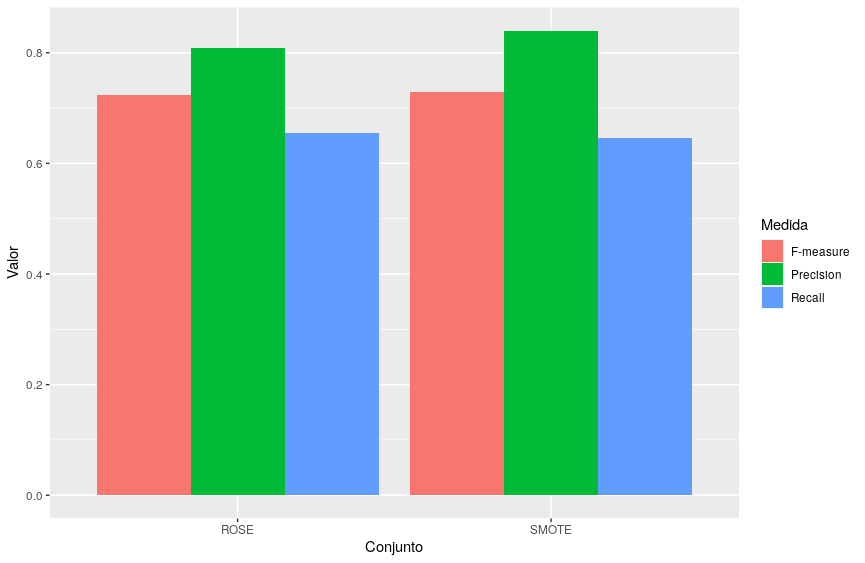
\includegraphics[width=\textwidth]{images/classification/lr-barplot.png}
    \caption{Medidas de calidad de la predicción realizada mediante regresión logística.}
    \label{fig:lr-barplot}
\end{figure}

\subsection{Perceptrón multicapa}
El segundo clasificador utilizado es el perceptrón multicapa. Estas redes
neuronales son ampliamente utilizadas en problemas de clasificación debido a su
capacidad para extraer características ocultas de los patrones del conjunto de
entrenamiento.

\begin{lstlisting}
# ROSE
mlp_control_rose <- trainControl(method = "repeatedcv", number = 10, repeats = 5)
mlp_model_rose <- train(
  isFraud ~ .,
  data = train_rose,
  method = "mlp",
  trControl = mlp_control_rose
)

mlp_prediction_rose <- predict(mlp_model_rose, val_rose, type = "raw")

# SMOTE
mlp_control_smote <- trainControl(method = "repeatedcv", number = 10, repeats = 5)
mlp_model_smote <- train(
  isFraud ~ .,
  data = train_smote,
  method = "mlp",
  trControl = mlp_control_smote
)

mlp_prediction_smote <- predict(mlp_model_smote, val_smote, type = "raw")
\end{lstlisting}

Es cierto que consumen más recursos que el otro clasificador usado, pero también
se podría esperar que se consiguieran resultados más precisos. En la figura
\ref{fig:mlp-barplot} se pueden ver estos resultados, que son incluso peores que
los obtenidos por el clasificador basado en regresión logística. Sí que podemos
destacar los resultados obtenidos para el conjunto de datos balanceado con
SMOTE. En este caso, vemos como la precisión es muy baja y la exhaustividad es
muy elevada. El clasificador es capaz de identificar muy bien los verdaderos
positivos del conjunto, pero también cuenta con un gran número de falsos
positivos. En resumen, sacamos de aquí que este clasificador tiende a clasificar
como fraude la mayoría de las transacciones.

\begin{figure}
    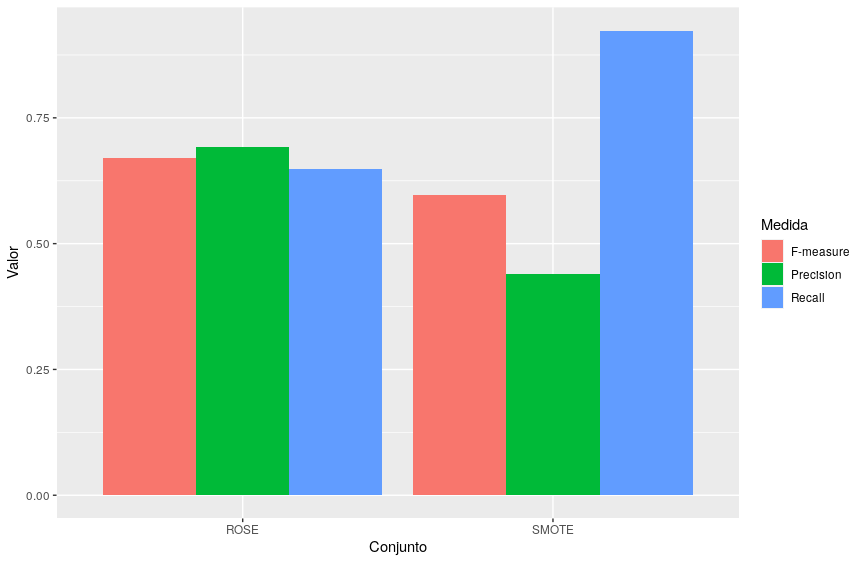
\includegraphics[width=\textwidth]{images/classification/mlp-barplot.png}
    \caption{Medidas de calidad de la predicción realizada por el perceptrón multicapa.}
    \label{fig:mlp-barplot}
\end{figure}

\subsection{Comparación}
Para comparar los clasificadores entre ellos, vamos a separar los resultados
obtenidos para el conjunto de datos al que se ha aplicado ROSE y al que se ha
aplicado SMOTE.

En la figura \ref{fig:rose-barplot}, tenemos los resultados de ambos
clasificadores sobre el conjunto de validación de ROSE. Apreciamos claramente
como la precisión ha sido menor con el perceptrón multicapa, mientras que la
exhaustividad se ha mantenido practicamente igual. En definitiva, los resultados
dados por el perceptrón han sido peores que los obtenidos con la regresión
logística.

En cuanto al conjunto de SMOTE, podemos ver los resultados de ambos
clasificadores en la figura \ref{fig:smote-barplot}. Aquí es donde tenemos los
resultados más dispares. Ya hemos explicado en el apartado anterior que los
resultados del perceptrón nos hacen ver que clasifica la mayoría de
transacciones como fraudulentas, lo que hace que no sea un clasificador fiable.
La regresión logística vuelve a ser mejor que el perceptrón, aunque sus
resultados tampoco son demasiado buenos.

\begin{figure}
    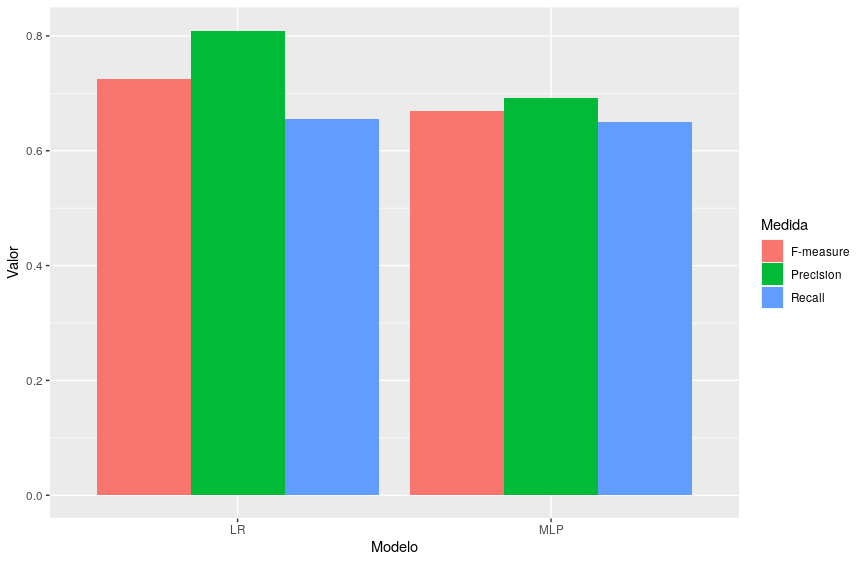
\includegraphics[width=\textwidth]{images/classification/rose-barplot.png}
    \caption{Medidas de calidad de las predicciones realizadas sobre el conjunto de datos ROSE.}
    \label{fig:rose-barplot}
\end{figure}

\begin{figure}
    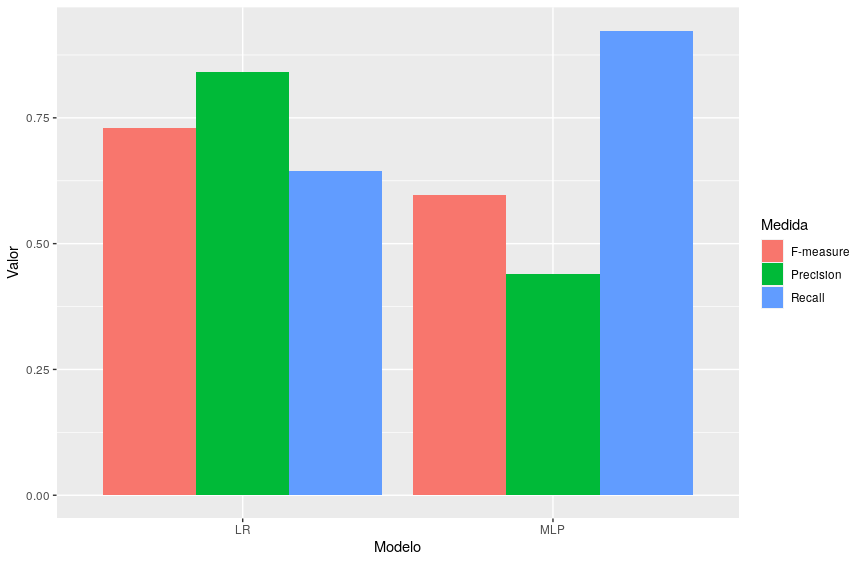
\includegraphics[width=\textwidth]{images/classification/smote-barplot.png}
    \caption{Medidas de calidad de las predicciones realizadas sobre el conjunto de datos SMOTE.}
    \label{fig:smote-barplot}
\end{figure}
